% This is sigproc-sp.tex -FILE FOR V2.6SP OF ACM_PROC_ARTICLE-SP.CLS
% OCTOBER 2002
%
% It is an example file showing how to use the 'acm_proc_article-sp.cls' V2.6SP
% LaTeX2e document class file for Conference Proceedings submissions.
% 
%----------------------------------------------------------------------------------------------------------------
% This .tex file (and associated .cls V2.6SP) *DOES NOT* produce:
%       1) The Permission Statement
%       2) The Conference (location) Info information
%       3) The Copyright Line with ACM data
%       4) Page numbering
%
%  However, both the CopyrightYear (default to 2002) and the ACM Copyright Data
% (default to X-XXXXX-XX-X/XX/XX) can still be over-ridden by whatever the author
% inserts into the source .tex file.
% e.g.
% \CopyrightYear{2003} will cause 2003 to appear in the copyright line.
% \crdata{0-12345-67-8/90/12} will cause 0-12345-67-8/90/12 to appear in the copyright line.
%
%
%---------------------------------------------------------------------------------------------------------------
% It is an example which *does* use the .bib file (from which the .bbl file
% is produced).
% REMEMBER HOWEVER: After having produced the .bbl file,
% and prior to final submission,
% you need to 'insert'  your .bbl file into your source .tex file so as to provide
% ONE 'self-contained' source file.
%
% Questions regarding SIGS should be sent to
% Adrienne Griscti ---> griscti@acm.org
%
% Questions/suggestions regarding the guidelines, .tex and .cls files, etc. to
% Gerald Murray ---> murray@acm.org 
%
% For tracking purposes - this is V2.6SP - OCTOBER 2002


\documentclass[12pt]{article}

\setlength{\oddsidemargin}{0in}
\setlength{\evensidemargin}{0in}
\setlength{\topmargin}{0in}
\setlength{\headheight}{0in}
\setlength{\headsep}{0in}
\setlength{\textwidth}{6in}
\setlength{\textheight}{9in}
\setlength{\parindent}{0in} 

\usepackage{graphicx} %For jpg figure inclusion
\usepackage{times} %For typeface
\usepackage{epsfig}
\usepackage{xcolor} %For Comments
%\usepackage[all]{xy}
\usepackage{float}
%\usepackage{subfigure} 
\usepackage{hyperref}
\usepackage{url}
\usepackage{parskip}
\usepackage{listings}

%% Elena's favorite green (thanks, Fernando!)
\definecolor{ForestGreen}{RGB}{34,139,34}
\definecolor{BlueViolet}{RGB}{138,43,226}
\definecolor{Coquelicot}{RGB}{255, 56, 0}
\definecolor{Teal}{RGB}{2,132,130}
%Uncomment this if you want to show work-in-progress comments
\newcommand{\comment}[1]{{\bf \tt  {#1}}}
% Uncomment this if you don't want to show comments
%\newcommand{\comment}[1]{}
% for color names see https://www.overleaf.com/learn/latex/Using_colors_in_LaTeX
\newcommand{\emcomment}[1]{\textcolor{ForestGreen}{\comment{Elena: {#1}}}}
\newcommand{\todo}[1]{\textcolor{blue}{\comment{To Do: {#1}}}}
\newcommand{\tkcomment}[1]{\textcolor{Teal}{\comment{Tristan: {#1}}}}
\newcommand{\jscomment}[1]{\textcolor{olive}{\comment{Jaydon: {#1}}}}
\newcommand{\jwcomment}[1]{\textcolor{violet}{\comment{John: {#1}}}}
%%%%%%%%%%%%%%%%%%%%%%%%%%%%%%%%%%%%%%%%%%

\begin{document}
\pagestyle{plain}
%
% --- Author Metadata here ---
%\conferenceinfo{WOODSTOCK}{'97 El Paso, Texas USA}
%\setpagenumber{50}
%\CopyrightYear{2002} % Allows default copyright year (2002) to be
%over-ridden - IF NEED BE. 
%\crdata{0-12345-67-8/90/01}  % Allows default copyright data
%(X-XXXXX-XX-X/XX/XX) to be over-ridden. 
% --- End of Author Metadata ---

\title{A beginner-friendly environment for exploring error messages in the Clojure programming language.}
%\subtitle{[Extended Abstract \comment{DO WE NEED THIS?}]
%\titlenote{}}
%
% You need the command \numberofauthors to handle the "boxing"
% and alignment of the authors under the title, and to add
% a section for authors number 4 through n.
%
% Up to the first three authors are aligned under the title;
% use the \alignauthor commands below to handle those names
% and affiliations. Add names, affiliations, addresses for
% additional authors as the argument to \additionalauthors;
% these will be set for you without further effort on your
% part as the last section in the body of your article BEFORE
% References or any Appendices.

\author{
Tristan Kalvoda, Elena Machkasova, Jaydon Stanislowski, and John Walbran\\
Computer Science Discipline \\
University of Minnesota Morris\\
Morris, MN 56267\\
kalvo007@umn.edu, elenam@umn.edu, stani152@umn.edu, walbr042@umn.edu
}
\date{}
\maketitle
\thispagestyle{empty}
%\alcomment{Should these say @morris.umn.edu?}

\section*{\centering Abstract}


\newpage
\setcounter{page}{1}

\section{Introduction}
The Clojure programming language is a functional language in the Lisp family, developed and released in 2007 
by Rich Hickey~\cite{Hickey:2008}. 
Clojure is implemented in Java, compiles to Java bytecode, and runs in the Java Virtual Machine (JVM), 
allowing programmers to use Java libraries directly from Clojure. 
However, unlike Java, it is a dynamically typed functional language with immutable data as a default (mutable data 
must be specifically declared).
Clojure quickly became known in industry. Even though the number of Clojure programmers is not a large percentage
of all developers (1.3\% of professional developers reported extensive use of Clojure), it remains one of the most admired languages (68.5\%) and is the 3rd highest-paying programming language, according to the 2024 Stack Overflow Developers Survey~\cite{survey}.

There is a long history of teaching Lisp as the first programming language, starting from the famous  ``Structure and Interpretation of Computer Programs'' curriculum~\cite{Abelson} and continuing with the introduction of the 
Racket programming language that provides a tiered system of Lisp-based beginner languages~\cite{Felleisen:2004,racket}. While Clojure is also a Lisp language and shares the benefits of focusing on development of functions that follow the structure of the data representation, some of Clojure's aspects make it more challenging than other Lisps for novice programmers. 

One such aspect is Clojure error messages: due to Clojure implementation via the underlying Java language, 
Clojure errors are Java exceptions. 
They frequently contain terminology intended for experienced developers, leaving out important context. 
As a result, what would otherwise be a powerful educational tool presents a difficult learning curve for new programmers.

%\emcomment{A 2-sentence overview of Babel, mention the name}
A project at UMN Morris, called Babel, aims at providing alternative beginner-friendly error messages and other tools that help beginner programmers to interpret Clojure errors. 
The current state of the project provides a tool to rewrite the majority of error messages into a clearer and more specific form - for example, specifying the erroneous arguments to functions. 
The challenge at this point lies in connecting this tool to a variety of possible ways of interacting with Clojure (via an interpreter or in IDE, for example). 
We also are working on providing features to give the users more resources and more control when they are receiving an error message. The resources include explanation of terminology (for example, what does the term ``hashmap'' refer to?), links to documentation for functions, etc. Giving users more control allows for optional expansion of some information, such as the stack trace. 
This work is still in progress. 
In this paper we discuss our approaches to tackling this task, demonstrate our current achievements, and discuss future directions. 

The rest of the paper is structured as following:
Section~\ref{sec:background} provides background on Clojure, its error messages, and the Clojure feature called {\it spec} that we utilize on our work. Section~\ref{sec:babel} discusses how Babel processes error messages. 
Section~\ref{sec:interactive} describes the interactive environment that we are developing, both from the implementation side and from the standpoint of design for the users. 
Section~\ref{sec:future} discusses future tasks and directions.  

\subsection{Related Work}\label{subsec:related}

Previous work on the topic of improving error messages in general for beginners~\cite{cosmetic} revealed that 
certain visual design choices can have a strong impact on a user's comprehension of error data. Dong and Khandwala found that, 
out of text coloring, increased white space, and collapsible components, adding whitespace to separate important sections of the 
error message helped to aid with understanding the most overall, and that employing theories of visual perception in the design 
of error messages help to improve their usability. 
We are using these insights as guidance for our approach.

A 2017 paper by Wrenn and Krishnamurthi~\cite{classifiers} on error handling in Racket, another Lisp-based programming language, 
suggests treating error messages as classifiers, using highlighting tools to mark up error messages. This is somewhat similar to 
our own approach in that we extract components of error messages and classify them using keywords to determine appropriate styling 
choices that make them more navigable to the end user.

An earlier paper on Racket~\cite{language} suggests that the vocabulary used in error messages plays a key role in the ability to
understand them, and students often have a hard time navigating technical language intended to point them to specific issues. This
knowledge is important to our own research, as native Clojure error messages often contain highly technical vocabulary as well, and 
we make an effort to replace such terminology with more universal language.

\section{Background}\label{sec:background}

\subsection{Clojure and its Error Messages}\label{subsec:clojure-errs}
%\emcomment{somewhere need to say something about Clojure syntax, in particular prefix notation}
Clojure syntax utilizes the prefix notation, common for Lisp languages: a Clojure expression is enclosed in parentheses that contain a function followed by its arguments. 
For example, \texttt{(/ 6 2)} denotes an expression $6 / 2$ and results in $3$. Clojure is dynamically typed, and no types are declared. 

In addition to lists (common in other Lisp languages), Clojure employs a variety of collections, such as vectors, hashmaps, and sets. 
It comes with a large number of predefined functions. Below we introduce collections and functions used in examples in this and subsequent sections. 
 
Vectors are enclosed in square brackets; commas between elements are optional and usually omitted. 
For example,  \texttt{[1 -1 0]} denotes a vector of three elements: $1, -1,$ and $0$. 
By convention Clojure uses \texttt{?} at the end of the names of predicates, i.e. functions that return a boolean. 
For example, \texttt{neg?} takes a number and returns \textit{true} if it's negative and \textit{false} otherwise.
Likewise, \texttt{even?} takes an integer and returns \textit{true} if it's even and \textit{false} otherwise.
A function \texttt{filter} is used to select elements of a vector, or another collection. 
It takes a predicate and  a collection and returns a collection with only the elements that satisfy the predicate. 
For example, \texttt{(filter neg? [1 -1 0])} would return a collection with only one element, $1$. 
A subtle point is that Clojure also allows passing just a predicate to \texttt{filter}, without a collection:  \texttt{(filter neg?)}. This returns a function that can be invoked on a vector at some later point. 
Since this use is allowed, the correct number of arguments for \texttt{filter} is one or two. 
%\emcomment{filter, neg?, even? - what else?}

	Clojure is a hosted language, running on the Java Virtual Machine (JVM), which is a bytecode interpreter that allows a program to run on any computer without needing to be rewritten for each one. 
	The JVM works by compiling code into bytecode, which it can then run. 
Clojure code can be loaded into the JVM from a file or directly via an interactive interpreter known as REPL, which stands for Read - Evaluate - Print - Loop. In our examples we assume that the code is entered into REPL. 
The REPL prompt is denoted with \texttt{=>}, and the Clojure response follows. 

When Clojure code is executed, it compiles into JVM bytecode, allowing it to use many of the features that the JVM provides, 
	but most importantly for the work presented here is that it uses the Java exception system for handling errors and when an exception is thrown in Clojure, it is a Java exception.

    
   An exception is an event or error that disrupts the normal flow of a program's execution. In Clojure, exceptions typically occur when something goes wrong, such as dividing by 
   zero or passing an inappropriate argument to a function. It's important to note that Clojure syntax errors will also result in an exception, because during the compilation of dynamically loaded Clojure code into JVM bytecode, 
   any syntax error will 
%prevent the code from being compiled and 
cause an exception.

   Error messages are generated when an exception occurs. They provide information about
   the type of error as well as where it happens, for example:

	\begin{figure}[h]
		\centering
		\begin{lstlisting}[breaklines=true, basicstyle=\ttfamily]
	=> (/ 9 0)
	Execution error (ArithmeticException) at user/eval1 (REPL:1).
	Divide by zero
		\end{lstlisting}
	\end{figure}

%Note: Clojure uses prefix notation, which is where the operator comes before the operands. that is why it is \texttt{(/ 9 0)}, not \texttt{(9 / 0)}.

The code is causing an error because it is trying to divide by zero, Let's break apart the default Clojure message:
	\begin{itemize}
		\item \texttt{ ArithmeticException } is the type of error that happens.
		\item \texttt{ user/eval1 (REPL:1) } is the location of the error; since for this example we assume that the code was directly typed into REPL, the location is REPL, line 1. 
%which is where the Clojure code is being typed and tested and it happened in the first line.
		\item \texttt{ Divide by zero } is the given description for the cause of the error.
	\end{itemize}
The error message is a part of a Java exception object that contains more information. 
%To get the most recent error message, you can use \texttt{*e}, which holds the latest exception object.

The exception object for \texttt{(/ 9 0)} contains the following information, represented as a nested Clojure hashmap, 
i.e. a collection of key/value pairs. The key names are preceded by \texttt{:} The exception typically contains a stack trace (see the keyword \texttt{:trace}) listing the sequence of function calls that resulted in the error. While our project includes a way of selecting the most helpful information in the stack trace, this paper is not focusing on the stack trace. 

	\begin{figure}[h]
		\centering
		\begin{lstlisting}[breaklines=true, basicstyle=\ttfamily]
#error {
	:cause "Divide by zero"
	:via
	[{:type java.lang.ArithmeticException
	  :message "Divide by zero"
	  :at [clojure.lang.Numbers divide "Numbers.java" 190]}]
	:trace
	[[clojure.lang.Numbers divide "Numbers.java" 190]
	... omitting 18 lines...
	 [clojure.main main "main.java" 40]]}

		\end{lstlisting}
	\end{figure}
	
%	The \texttt{ex-triage} function uses an exception object to analyze errors and obtain information on the error's phase, cause, and location.
%	When an exception is thrown, Babel retrieves this exception object and uses \texttt{ex-triage} to interpret the error
%	We use the exception object in the \texttt{ex-triage} function to help interpret exceptions, which returns an analysis of the phase, error, cause, and location of an error.
%	the phase information in the \texttt{ex-triage} lets us know when the exception occurs. 

In addition to the above information, the exception contains the phase of Clojure execution when the exception occurred. For example, in the earlier case of the divide by zero error, the exception occurs in the execution phase. 
%
	%\tkcomment{: and line from :line are being seperated by line wrapping}
%
%	\begin{figure}[h]
%		\centering
%		\begin{lstlisting}[breaklines=true, basicstyle=\ttfamily]
%user=> (clojure.main/ex-triage(Throwable->map *e))
%#:clojure.error{:class java.lang.ArithmeticException, :line 1, :cause "Divide by zero", :symbol user/eval1, :phase :execution}
%		\end{lstlisting}
%	\end{figure}
Since an error can occur at any point in the Read-Evaluate-Print-Loop, there are several possibilities of the phase. Below we list some of them:
	\begin{figure}[h]
		\centering
		\begin{tabular}{|c|l|}
			\hline
			\textbf{Phase} & \textbf{Description} \\
			\hline
			:read-source & Error while reading characters at the REPL or from a source file. \\
			:compile-syntax-check & Syntax error caught during compilation. \\
			:execution & Any errors thrown at execution time. \\
			:read-eval-result & Error thrown while reading the result of execution. \\
			:print-eval-result & Error thrown while printing the result of execution. \\
			\hline
		\end{tabular}
	\end{figure}
Knowing the phase of the evaluation is helpful for detecting what kind of error has occurred and what information the user would benefit from.

\tkcomment{Abrupt shift here}
\emcomment{Maybe move to before division by zero?}
As an example of one such mistake, a novice to Clojure might write the expression below, instead of the correct 
version \texttt{(filter neg? [1 -1 0])} described above:
\begin{verbatim}
(filter neg? 1 -1 0)
\end{verbatim}

This causes an error, because the filter function was expecting either 1 or 2 arguments,
 which should be a predicate or a predicate and a collection. Here 1, -1, and 0 are not in a collection. 
 Instead, they are being passed as separate arguments, which causes the function to be overloaded with inputs it doesn't expect.

 \begin{figure}[h]
	\centering
	\begin{lstlisting}[breaklines=true, basicstyle=\ttfamily]
Execution error (ArityException) at user/eval1 (REPL:1).
Wrong number of args (4) passed to: clojure.core/filter
	\end{lstlisting}
\end{figure}
The correct way to use filter here would be:
\begin{verbatim}
(filter neg? [1 -1 0])
\end{verbatim}
%\tkcomment{Should I mention that the actual error could be a syntax error, because it is missing the [] around the extra arguments}
%\emcomment{No, since there is no way Clojure would be able to detect this.}
 Clojure presents this error as an {\it ArityException}, referring to the number of arguments of the function. 
 The message is cryptic for beginners, especially without the documentation.

\subsection{Clojure Spec}\label{subsec:spec}
%\emcomment{Elena's section.}
Clojure \textit{spec} is an addition to Clojure first released around 2016~\cite{spec-overview}.
It is a set of features that allow setting specifications, particularly for functions, that are checked before the function call. 
These specifications typically include the number and types of arguments, although they may include other conditions.
The flexible nature of spec allows programmers to choose what parameters to check and, to a degree, what information will be communicated about why the arguments failed to satisfy spec.

As an example, one may specify that a function \texttt{f} takes no fewer than 2 and no more than 4 arguments, the first argument must be a non-negative integer, and the second one must be sequence. 
Types (or any other conditions) are specified as predicates. 
For example, we can require that the first argument of \texttt{f} satisfy both \texttt{number?} and \texttt{pos?} predicates, and the second satisfies \texttt{seq?} (a predicate that determines if a Clojure object is a sequence).
Any existing Clojure predicate can be used, or the user can write their own. 

If arguments not satisfying the spec are passed to the function, a spec error will occur. 
A spec error is an exception of the type \texttt{clojure.lang.ExceptionInfo} that contains data describing the error, including the failed predicate.
For example, if the second argument of the function 
\texttt{f} above is a number $5$, and not a sequence, the error message states that it failed the predicate \texttt{seq?}
Even more importantly, the argument that's causing the error (in this case $5$) will be included in the spec error message.

Without using spec, the error message would be a Java \texttt{ClassCastException} that doesn't report the value of the failing argument, only the incompatible types. 
The more detailed information provided by spec allows us to make error messages more understandable to novice programmers, as described in Section~\ref{subsec:overview}. 

\section{Babel Project}\label{sec:babel}
\subsection{Overview of the Project}\label{subsec:overview}
%\jscomment{Jaydon's subsection}
%\emcomment{Explain the difference in prompts: user vs babel.middleware}
Our research project, Babel, is a tool intended to help novice programmers understand Clojure errors. It does this by providing learners with substitute error messages that describe code problems in simpler terms, replacing the unfamiliar jargon and low-level clutter of native error messages. For example, the error message produced via the function call below: \emcomment{explain what count is}

\begin{lstlisting}[breaklines=true, basicstyle=\ttfamily]
    => (count 1)
    Execution error (UnsupportedOperationException) at user/eval1529 (REPL:1).
    count not supported on this type: Long
\end{lstlisting}
    
is transformed into a new message, replacing the reference to the internal type \verb|Long| and removing details about the Java exception object and irrelevant internal information:

\begin{lstlisting}[breaklines=true, basicstyle=\ttfamily]
    => (count 1)
    Function count does not allow a number as an argument in this position.

    In Clojure interactive session on line 1.
    Call sequence:
    [Clojure interactive session (repl)]
\end{lstlisting}

Babel creates error messages like these through simple analysis of the native error's Java exception class and message contents, and one could argue that for cases like these, the native error message suffices. However, for more complicated problems, such as incorrect calls to functions or malformed arguments, Clojure's messages get more difficult to parse. Consider the previous error: \emcomment{"previous" should be "earlier", with a subsection reference.} 

\begin{lstlisting}[breaklines=true, basicstyle=\ttfamily]
    => (filter neg? 1 -1 0)
    Execution error (ArityException) at user/eval1540 (REPL:1).
    Wrong number of args (4) passed to: clojure.core/filter
\end{lstlisting}

In these situations, it would be ideal to have a detailed explanation of what the offending arguments in the function call are, and what was expected. This is where Babel makes use of the Clojure spec library in its error reporting.

By employing specs on core Clojure functions, it is possible to explicitly determine the correct form of a function call and how the function was used incorrectly. Using spec, we know that the \verb|filter| function must take a predicate and, optionally, a collection, therefore expecting one or two arguments. With Babel, the above error message is replaced as follows:

\begin{lstlisting}[breaklines=true, basicstyle=\ttfamily]
    => (filter neg? 1 -1 0)
    Wrong number of arguments in (filter neg? 1 -1 0): the function filter expects one or two arguments but was given four arguments.
    In Clojure interactive session on line 1.
    Call sequence:
    [Clojure interactive session (repl)]
\end{lstlisting}

Our project presently includes specs for many pre-existing Clojure functions and rewrites a majority of potential Clojure errors that cannot employ spec (such as divisions by zero, unmatched delimiters, etc). With much of the internal work done at this stage of the project, our focus is now on the potential of third party tools to display modified error messages in an interactive viewer that will allow beginner programmers to explore them more dynamically and familiarize themselves with how Clojure itself handles error data, enabling them to view the data in a more organized way and easily explore related documentation.

\emcomment{Also need to include:
Babel constructs its error messages by intercepting exception objects directly from REPL , hooking an observer to a running instance of a REPL server.}

\subsection{Classifying Error Messages}\label{subsec:classification}

Errors can be categorized broadly into spec errors and non-spec errors
\begin{itemize}

	\item Spec errors occur when the data does not conform to the expected specification defined using the clojure.spec library. They are triggered when the data doesn't meet the specific requirements created for a certain function or process.
	
	\item Non-spec errors occur when errors happen outside of the clojure.spec system. They are typically runtime errors, such as division by zero or any other errors that arise during program execution

\end{itemize}

Error messages can also be classified by their properties, some notable properties that we look at are Error Types, Levels of Nesting, and Phase.
\begin{itemize}
	\item Grouping by error types or subtypes can help find patterns in errors that make it easier to prescribe solutions to errors, based off of similar error types.
	\item Grouping by levels of nesting and the order in which errors occur provides more insight into the path the error took before it becomes visible, helping us understand the sequence of failures.
	\item Classifying by phase (such as :read-source, :execution, and :print-eval-result) offers additional context about when and where the error occurred.
\end{itemize}
Using the above in conjuction with each other would give greater ability to find and resolve errors.

\begin{itemize}

    \item \textbf{Babel Messages vs. Messages from Dictionary} \\
    \begin{itemize}
        \item LazySeq messages not caught in spec because worried that catching and printing at the point will change the order of eval (these are caught in the print phase) -- key decisions we made with our spec.
    \end{itemize}

    \item \textbf{Documenting Errors} \\
    Error on the receiving end and how to get where it came from.

    \item \textbf{How to Get Useful Information from Error?} \\
    Reverse-engineered through things like nested errors.

\end{itemize}
\tkcomment{Tristan's subsection}

\section{Adding Visual Interactive Environment}\label{sec:interactive}

We explore using the third-party Morse viewer as a supplementary way to interactively present error information in a better, more beginner-friendly format.
This provides an interactive, visual layer of error message presentation on top of the existing terminal error message display.
For instance, unlike default Clojure error messages, Babel uses monospace font for code snippets, and highlight function names with color coding. 
Additionally, for spec errors, Babel will generate the link to the documentation of the function where the error occurred.

Morse is a tool designed for data exploration and visualization.
While it was originally designed to help experienced developers navigate large datasets and projects, 
it provides tools and extensibility to be curated with a beginner audience in mind.
Morse uses a system of customizable viewers to achieve its data visualization.
Each view is individually designed to display a specific data structure based on given conditions.

\subsection{Running a Babel Session with Morse}\label{subsec:babel-w-morse}

By default, the Clojure REPL does not expose the correct hooks to effectively manipulate the data from error messages.
In order to get around this, initializing Babel within an existing REPL session, using the \texttt{(babel/init)} function, creates a new custom sub-REPL above the existing session.
Creating a sub-REPL allows us to configure the behavior attached to the following hooks:
\begin{itemize}
	\item \texttt{:init} Defines the initialization behavior of the sub-repl. 
		In Babel, this starts a new Morse session connected to the new REPl.
	\item \texttt{:eval} Defines the behavior whenever a command is executed within the REPL. 
		In Babel, this taps the command into an atom, and evaluates the command within both Morse and the REPL.
	\item \texttt{:caught} Defines the behavior on exception.
		In Babel, this processes the error as described previously, 
			and passes the following information about the error to Morse to be displayed in a custom viewer:
			\begin{itemize}
				\item The last command entered, read from an atom that is updated at evaluation.
				\item The location in the environment where the error occurred. In the REPL, this resolves to "Clojure Interactive Session".
				\item A vector of pairs containing the error message produced by Babel, with labels associated with each segment denoting its type for formatting.
				\item The url to the documentation of the function called that caused the error. 
			\end{itemize}
\end{itemize}
Once the sub-REPL is initialized, the use can then use the sub-REPL as normal, but with the addition of Babel error messages when applicable in the terminal, and a parallel Morse viewer.

\jwcomment{Make more explicit comment about vector labelling.}

%\jwcomment{There will be a diagram for this later.}

\subsection{Designing Morse Viewers}\label{subsec:Morse-Viewers}
Morse viewers can be created to have custom behavior around certain data.
Creating a new viewer in Morse requires the following:
\begin{itemize}
	\item A predicate defining the constraints of the data that can be displayed in the viewer.
	\item The graphical format of the view to be displayed. This is built with the JavaFX library. 
\end{itemize}
The Babel viewer takes a map of input data as input, and defines the predicate for the viewer by checking for a map with the necessary fields.
For the formatting definition, Babel uses the built-in \texttt{WebView} object in order to format the error data with an HTML template,
enabling us to leverage the large, robust tools of HTML and CSS to define the visuals of the error messages.

\jwcomment{John's subsection}

\subsection{Exploring Design of Error Messages Interface}\label{subsec:interface}
\emcomment{TBD}

An example of the error presentation for Babel is shown in~\ref{fig:babelview}, showing the error message for the command \texttt{(even? 1 2)}. 
Code segments are displayed as monospace and isolated. Additionally, function names within the body of the error message are color coded. 
\begin{figure}
	\centering
	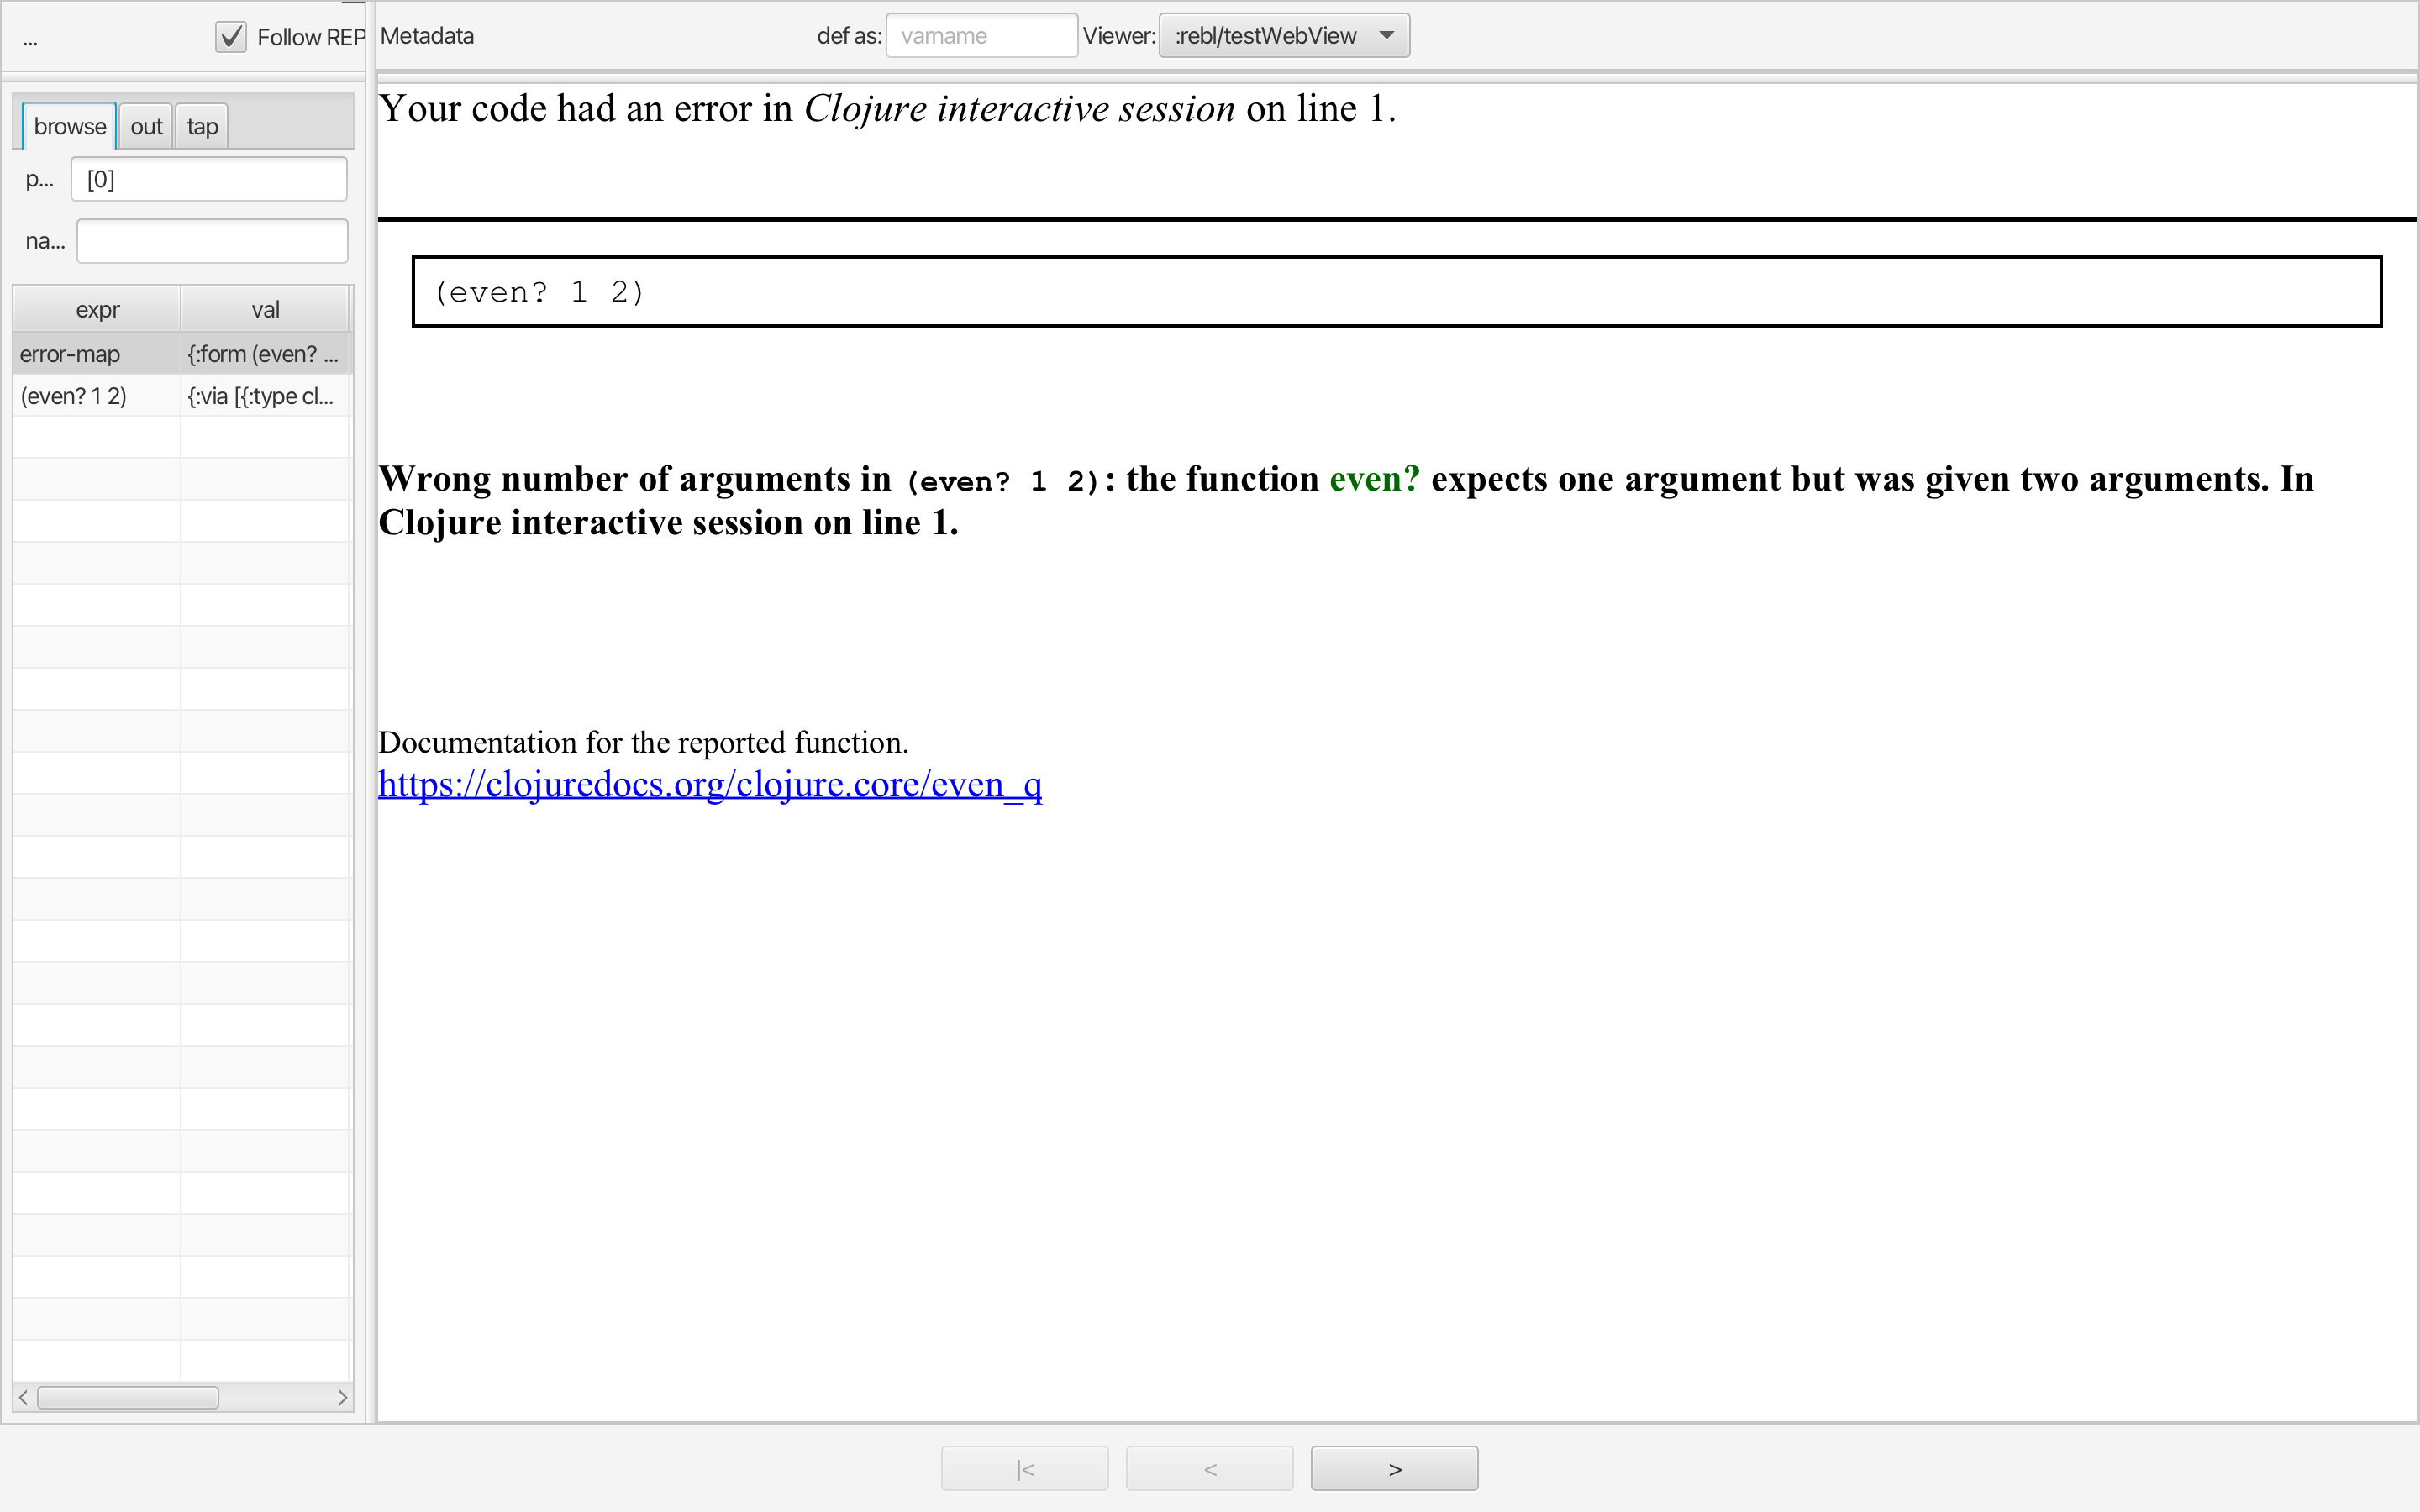
\includegraphics[width=\linewidth]{resources/BabelViewerExample.png}
	\caption{Morse visualization of the arity error on \texttt{(even?)} with too many arguments (right), with session evaluation history (left).}
	\label{fig:babelview}
\end{figure}

\section{Current State and Future Work}\label{sec:conclusion}

\emcomment{Interaction in a session with multiple error messages.}

\jscomment{I'm not sure if I've used Morse enough to write about the above in the time span that I have.}

As the project stands right now, many features of Morse are still in active development. For example, the ability to hover over specific terms used in error message for their definitions as well as to navigate collapsible stack traces would be useful for making the tool more interactive and helping beginners learn.

In the future, we would like to conduct usability studies with the interactive tools offered by Morse, after we have developed the tool enough to cover more of Babel's capabilities. Allowing research participants to experiment with the tool for learning Clojure would help drive the direction of the project and improve upon the design choices. We would also like to explore IDE integration as a potential avenue of development for Morse, in order to make the tool more useful for learning to code as a whole.

\bibliographystyle{acm}
\bibliography{mics2025}

\end{document}
